\documentclass[10,portrait]{article}
\usepackage{lmodern}
\usepackage{amssymb,amsmath}
\usepackage{ifxetex,ifluatex}
\usepackage{fixltx2e} % provides \textsubscript
\ifnum 0\ifxetex 1\fi\ifluatex 1\fi=0 % if pdftex
  \usepackage[T1]{fontenc}
  \usepackage[utf8]{inputenc}
\else % if luatex or xelatex
  \ifxetex
    \usepackage{mathspec}
  \else
    \usepackage{fontspec}
  \fi
  \defaultfontfeatures{Ligatures=TeX,Scale=MatchLowercase}
\fi
% use upquote if available, for straight quotes in verbatim environments
\IfFileExists{upquote.sty}{\usepackage{upquote}}{}
% use microtype if available
\IfFileExists{microtype.sty}{%
\usepackage[]{microtype}
\UseMicrotypeSet[protrusion]{basicmath} % disable protrusion for tt fonts
}{}
\PassOptionsToPackage{hyphens}{url} % url is loaded by hyperref
\usepackage[unicode=true]{hyperref}
\PassOptionsToPackage{usenames,dvipsnames}{color} % color is loaded by hyperref
\hypersetup{
            pdftitle={Using Github for research and life},
            colorlinks=true,
            linkcolor=blue,
            citecolor=red,
            urlcolor=blue,
            breaklinks=true}
\urlstyle{same}  % don't use monospace font for urls
\usepackage[margin=1in]{geometry}
\usepackage[]{biblatex}
\usepackage{color}
\usepackage{fancyvrb}
\newcommand{\VerbBar}{|}
\newcommand{\VERB}{\Verb[commandchars=\\\{\}]}
\DefineVerbatimEnvironment{Highlighting}{Verbatim}{commandchars=\\\{\}}
% Add ',fontsize=\small' for more characters per line
\usepackage{framed}
\definecolor{shadecolor}{RGB}{248,248,248}
\newenvironment{Shaded}{\begin{snugshade}}{\end{snugshade}}
\newcommand{\KeywordTok}[1]{\textcolor[rgb]{0.13,0.29,0.53}{\textbf{#1}}}
\newcommand{\DataTypeTok}[1]{\textcolor[rgb]{0.13,0.29,0.53}{#1}}
\newcommand{\DecValTok}[1]{\textcolor[rgb]{0.00,0.00,0.81}{#1}}
\newcommand{\BaseNTok}[1]{\textcolor[rgb]{0.00,0.00,0.81}{#1}}
\newcommand{\FloatTok}[1]{\textcolor[rgb]{0.00,0.00,0.81}{#1}}
\newcommand{\ConstantTok}[1]{\textcolor[rgb]{0.00,0.00,0.00}{#1}}
\newcommand{\CharTok}[1]{\textcolor[rgb]{0.31,0.60,0.02}{#1}}
\newcommand{\SpecialCharTok}[1]{\textcolor[rgb]{0.00,0.00,0.00}{#1}}
\newcommand{\StringTok}[1]{\textcolor[rgb]{0.31,0.60,0.02}{#1}}
\newcommand{\VerbatimStringTok}[1]{\textcolor[rgb]{0.31,0.60,0.02}{#1}}
\newcommand{\SpecialStringTok}[1]{\textcolor[rgb]{0.31,0.60,0.02}{#1}}
\newcommand{\ImportTok}[1]{#1}
\newcommand{\CommentTok}[1]{\textcolor[rgb]{0.56,0.35,0.01}{\textit{#1}}}
\newcommand{\DocumentationTok}[1]{\textcolor[rgb]{0.56,0.35,0.01}{\textbf{\textit{#1}}}}
\newcommand{\AnnotationTok}[1]{\textcolor[rgb]{0.56,0.35,0.01}{\textbf{\textit{#1}}}}
\newcommand{\CommentVarTok}[1]{\textcolor[rgb]{0.56,0.35,0.01}{\textbf{\textit{#1}}}}
\newcommand{\OtherTok}[1]{\textcolor[rgb]{0.56,0.35,0.01}{#1}}
\newcommand{\FunctionTok}[1]{\textcolor[rgb]{0.00,0.00,0.00}{#1}}
\newcommand{\VariableTok}[1]{\textcolor[rgb]{0.00,0.00,0.00}{#1}}
\newcommand{\ControlFlowTok}[1]{\textcolor[rgb]{0.13,0.29,0.53}{\textbf{#1}}}
\newcommand{\OperatorTok}[1]{\textcolor[rgb]{0.81,0.36,0.00}{\textbf{#1}}}
\newcommand{\BuiltInTok}[1]{#1}
\newcommand{\ExtensionTok}[1]{#1}
\newcommand{\PreprocessorTok}[1]{\textcolor[rgb]{0.56,0.35,0.01}{\textit{#1}}}
\newcommand{\AttributeTok}[1]{\textcolor[rgb]{0.77,0.63,0.00}{#1}}
\newcommand{\RegionMarkerTok}[1]{#1}
\newcommand{\InformationTok}[1]{\textcolor[rgb]{0.56,0.35,0.01}{\textbf{\textit{#1}}}}
\newcommand{\WarningTok}[1]{\textcolor[rgb]{0.56,0.35,0.01}{\textbf{\textit{#1}}}}
\newcommand{\AlertTok}[1]{\textcolor[rgb]{0.94,0.16,0.16}{#1}}
\newcommand{\ErrorTok}[1]{\textcolor[rgb]{0.64,0.00,0.00}{\textbf{#1}}}
\newcommand{\NormalTok}[1]{#1}
\usepackage{graphicx,grffile}
\makeatletter
\def\maxwidth{\ifdim\Gin@nat@width>\linewidth\linewidth\else\Gin@nat@width\fi}
\def\maxheight{\ifdim\Gin@nat@height>\textheight\textheight\else\Gin@nat@height\fi}
\makeatother
% Scale images if necessary, so that they will not overflow the page
% margins by default, and it is still possible to overwrite the defaults
% using explicit options in \includegraphics[width, height, ...]{}
\setkeys{Gin}{width=\maxwidth,height=\maxheight,keepaspectratio}
\IfFileExists{parskip.sty}{%
\usepackage{parskip}
}{% else
\setlength{\parindent}{0pt}
\setlength{\parskip}{6pt plus 2pt minus 1pt}
}
\setlength{\emergencystretch}{3em}  % prevent overfull lines
\providecommand{\tightlist}{%
  \setlength{\itemsep}{0pt}\setlength{\parskip}{0pt}}
\setcounter{secnumdepth}{0}
% Redefines (sub)paragraphs to behave more like sections
\ifx\paragraph\undefined\else
\let\oldparagraph\paragraph
\renewcommand{\paragraph}[1]{\oldparagraph{#1}\mbox{}}
\fi
\ifx\subparagraph\undefined\else
\let\oldsubparagraph\subparagraph
\renewcommand{\subparagraph}[1]{\oldsubparagraph{#1}\mbox{}}
\fi

% set default figure placement to htbp
\makeatletter
\def\fps@figure{htbp}
\makeatother


\title{Using Github for research and life}
\author{Matthew
Malishev\textsuperscript{1}*\\[2\baselineskip]\emph{\textsuperscript{1}
Department of Biology, Emory University, 1510 Clifton Road NE, Atlanta,
GA, USA, 30322}}
\date{}

\begin{document}
\maketitle

{
\hypersetup{linkcolor=black}
\setcounter{tocdepth}{4}
\tableofcontents
}
\newpage   

Date: 2018-11-13\\
R version: 3.5.0\\
*Corresponding author:
\href{mailto:matthew.malishev@gmail.com}{\nolinkurl{matthew.malishev@gmail.com}}\\
This document can be found at \url{https://github.com/darwinanddavis}\\
\newpage  

\subsection{Install git}\label{install-git}

Install git on your computer following the instructions
\href{https://git-scm.com/book/en/v2/Getting-Started-Installing-Git}{here}.

Once git is on your computer, you can now access its features using
either just your local computer for version control or your Github
account.

\subsection{Create a Github account}\label{create-a-github-account}

Create your new Github account \href{https://github.com/}{here}. Some
tips on creating an account:

\begin{itemize}
\tightlist
\item
  Choose a username that you plan to keep. Something that represents
  your professional acumen, e.g.~not ``matt\_loves\_hiphop86''\\
  \hspace*{0.333em}
\item
  Github is universal and really useful. You can connect to programming,
  troubleshooting, userX sites, and coding libraries, e.g.~CodePen,
  using your Github account, so plan for longevity.\\
  \hspace*{0.333em}
\end{itemize}

Feel free to navigate my personal Github page. Everything is publicly
available.

\url{www.github.com/darwinanddavis}

Some essential elements of your Github page:

\begin{itemize}
\tightlist
\item
  Your repositories. This is where you store your online information.\\
  \hspace*{0.333em}
\item
  Your gits. These are the digital footprints of your changes. We use
  this for
  \href{https://git-scm.com/book/en/v2/Getting-Started-About-Version-Control}{version
  control}.\\
  \hspace*{0.333em}
\item
  Your README.md file. This tells users what your repo contains,
  instructions for running code, troubleshooting, version control, links
  to external web sources, and other git specific elements, such as
  program/package versions.\\
  \hspace*{0.333em}
\end{itemize}

Here are some screenshots of what you'll see on your own github page.

\begin{figure}
\centering
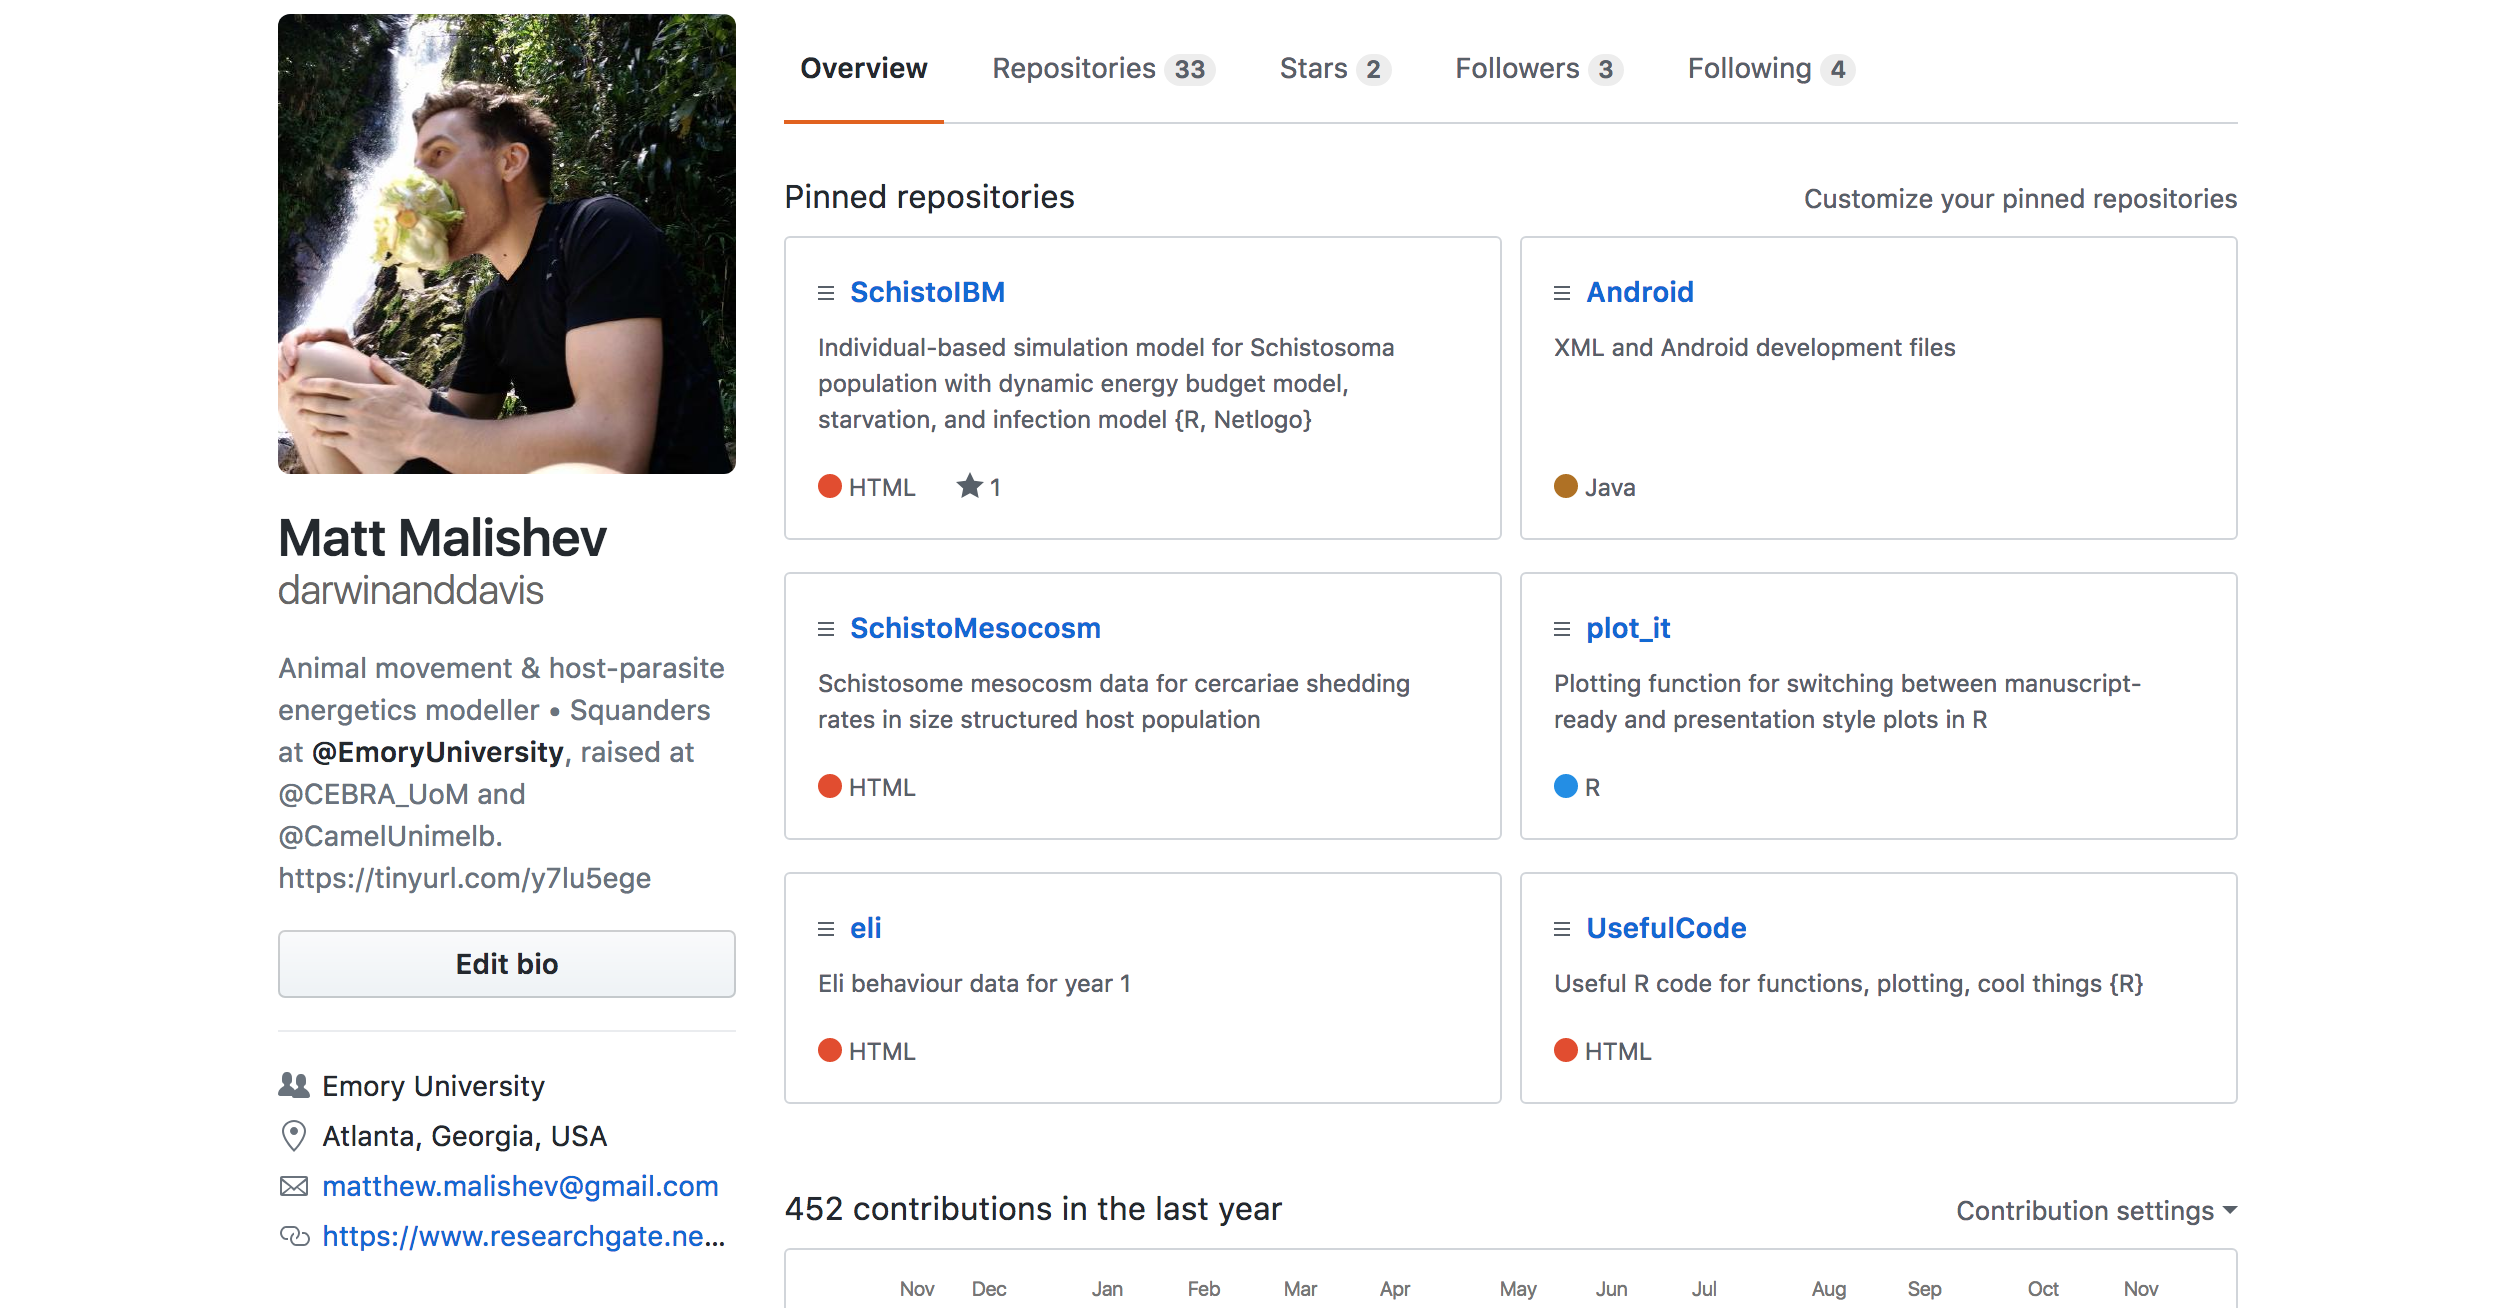
\includegraphics{loadingpage.png}
\caption{Github loading page}
\end{figure}

\begin{figure}
\centering
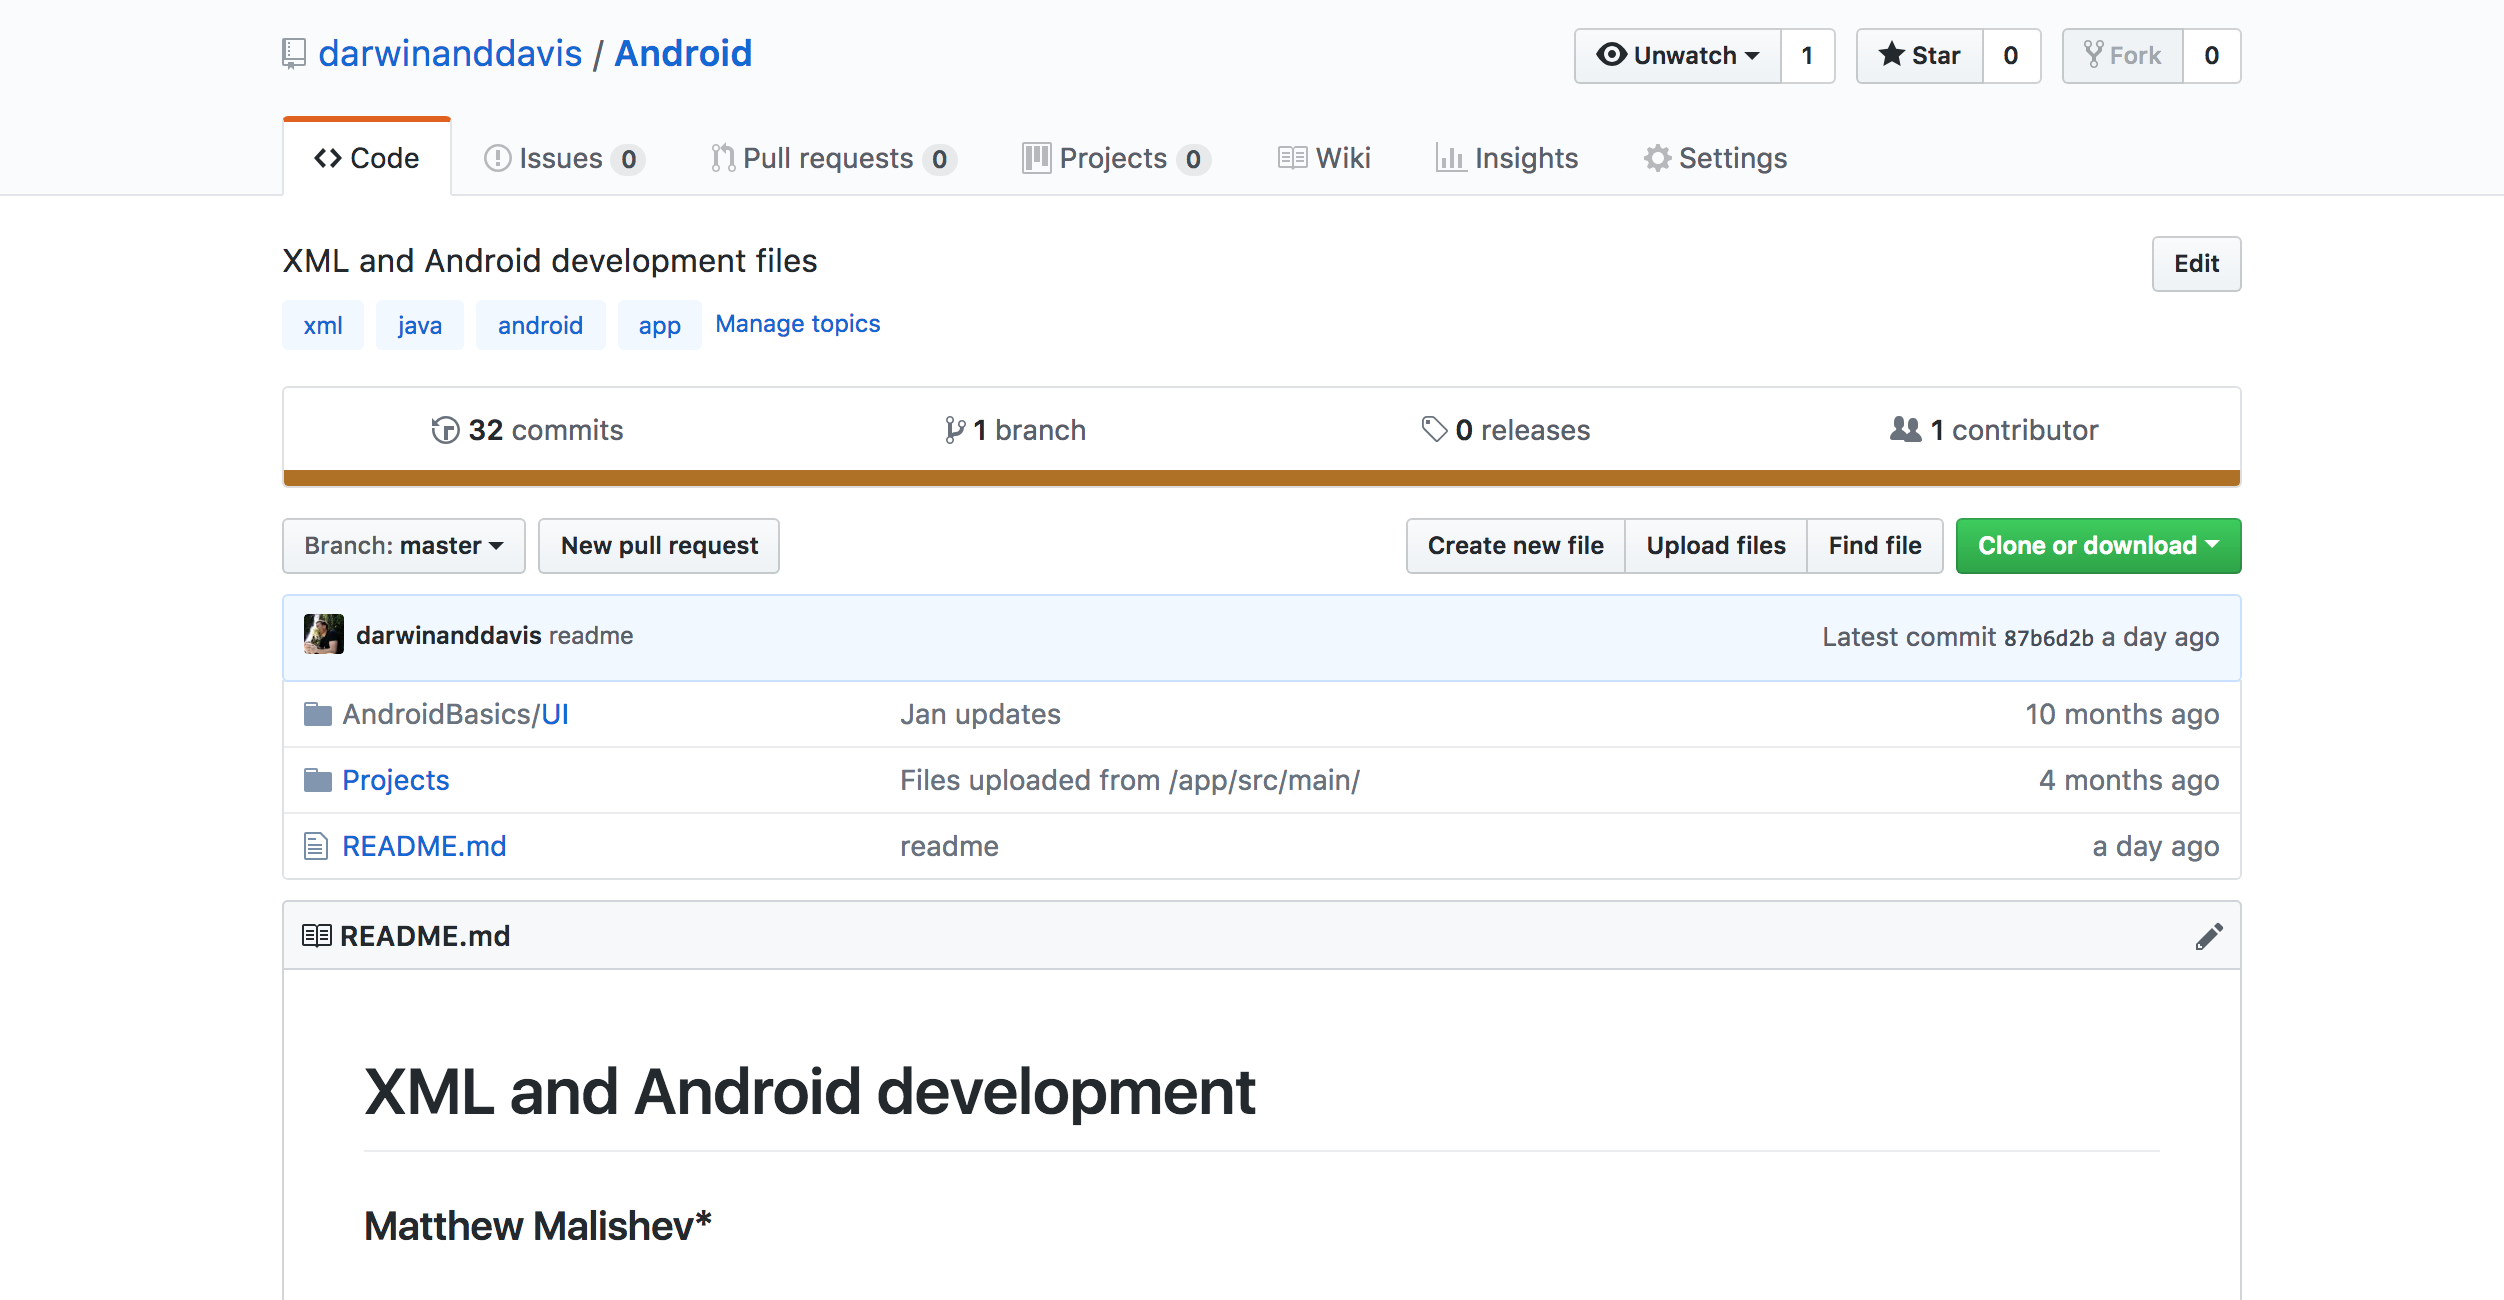
\includegraphics{repopage.png}
\caption{Repository loading page}
\end{figure}

\begin{figure}
\centering
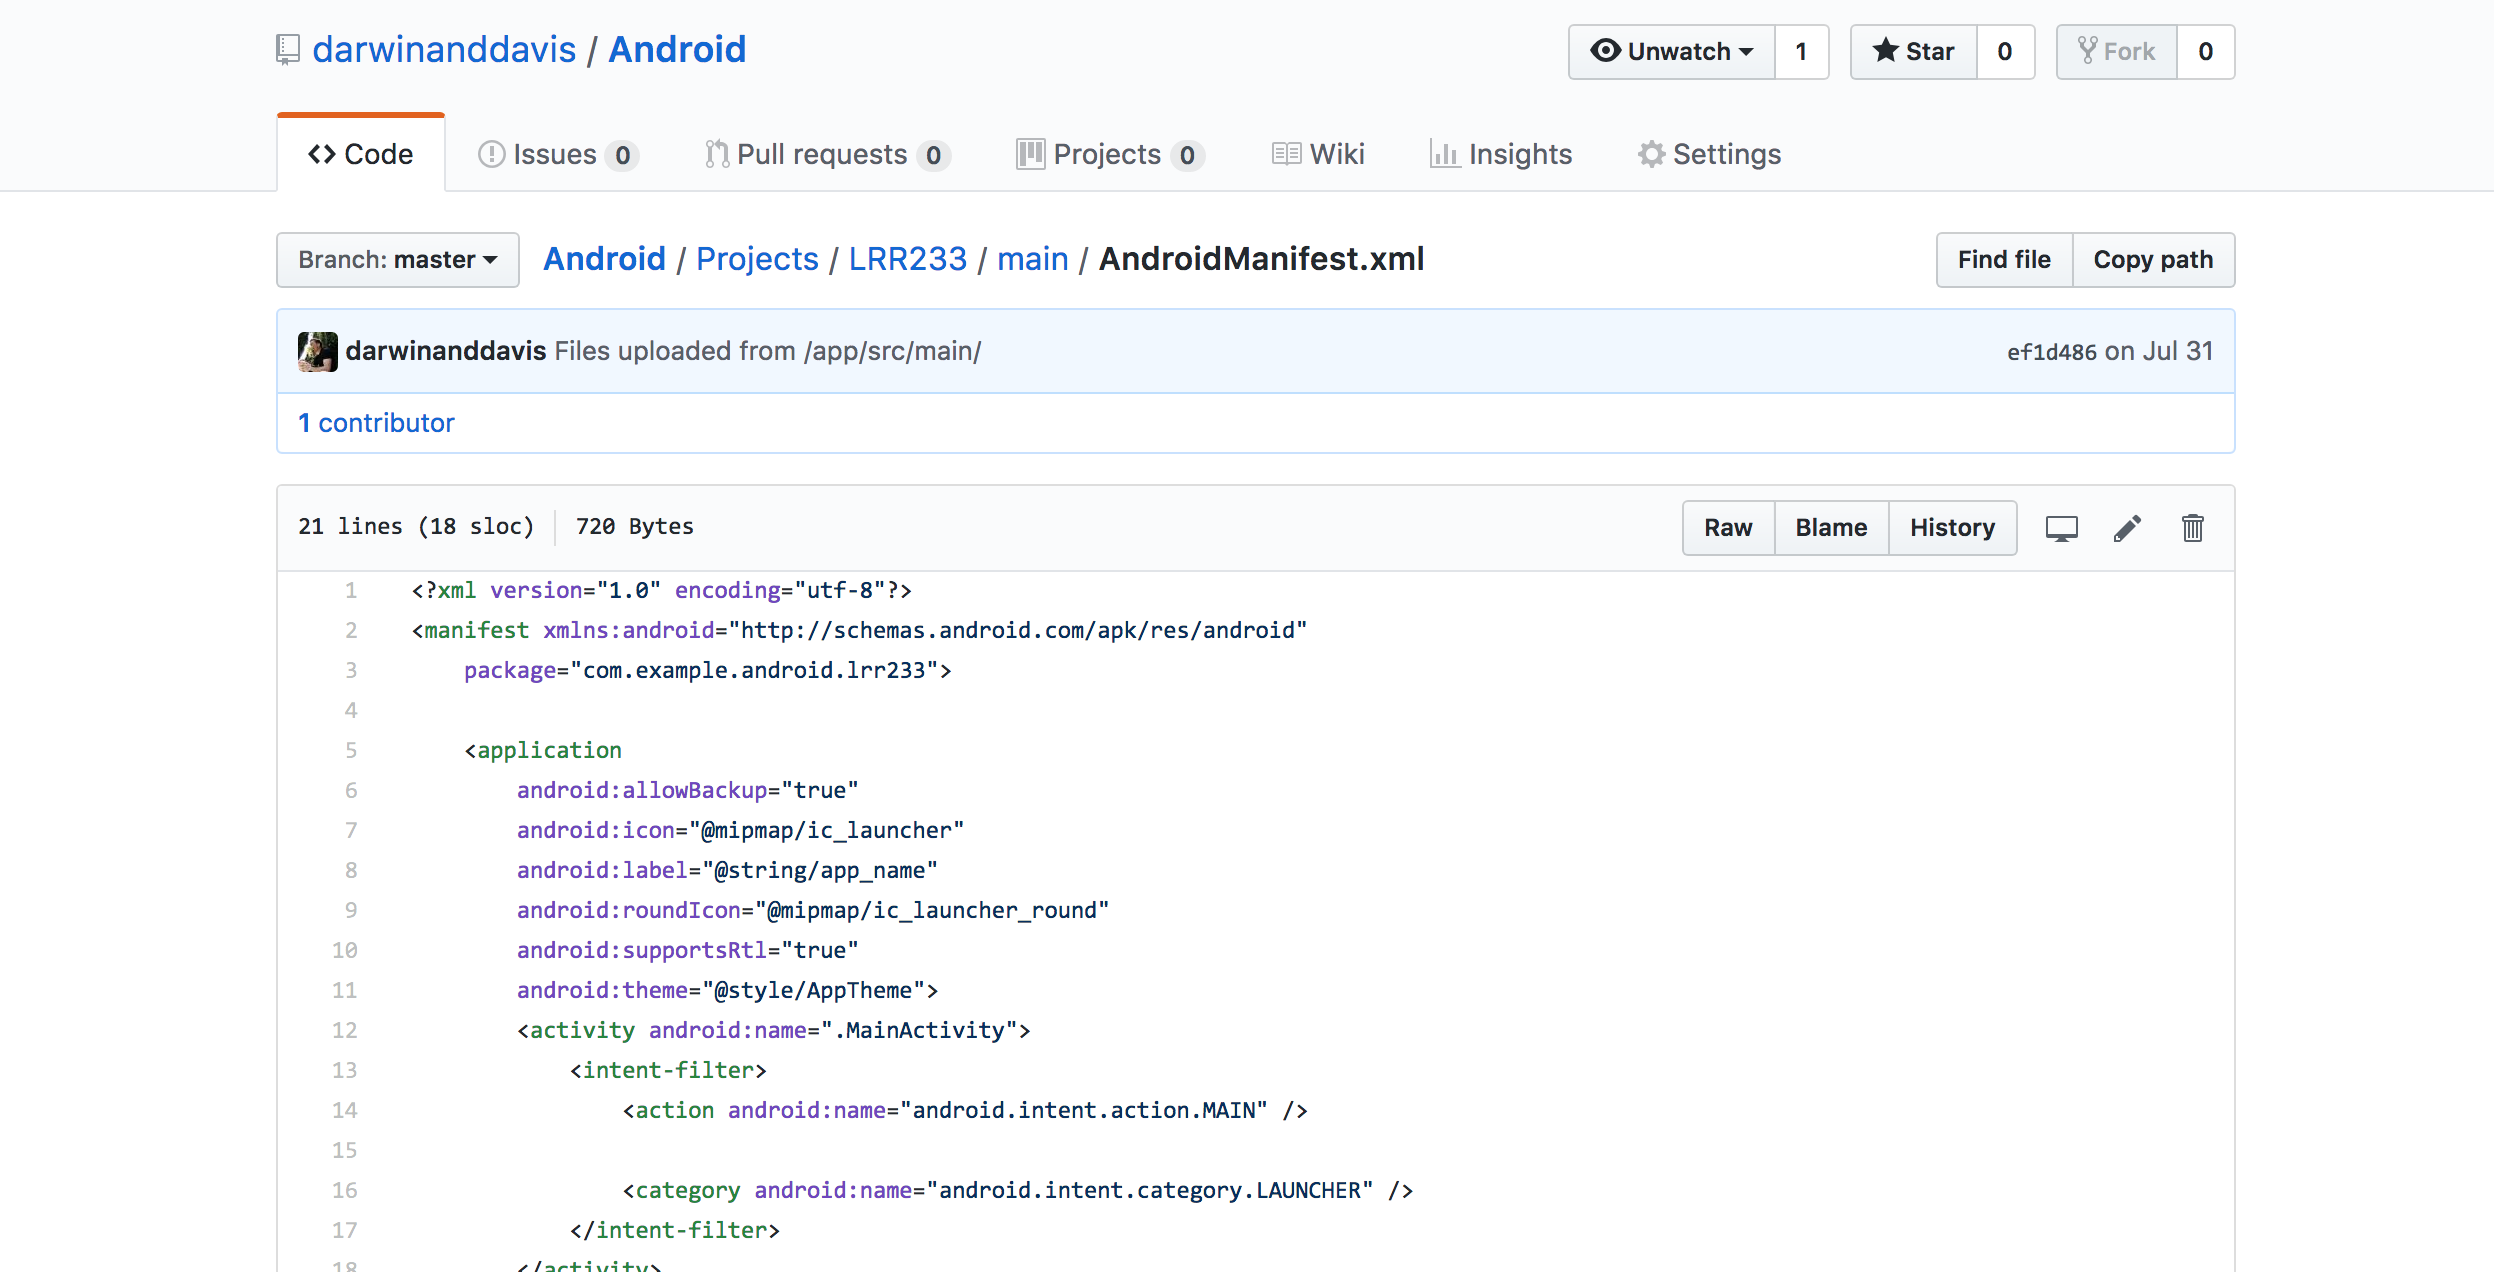
\includegraphics{filepage.png}
\caption{Inside of a file in a repository}
\end{figure}

\begin{figure}
\centering
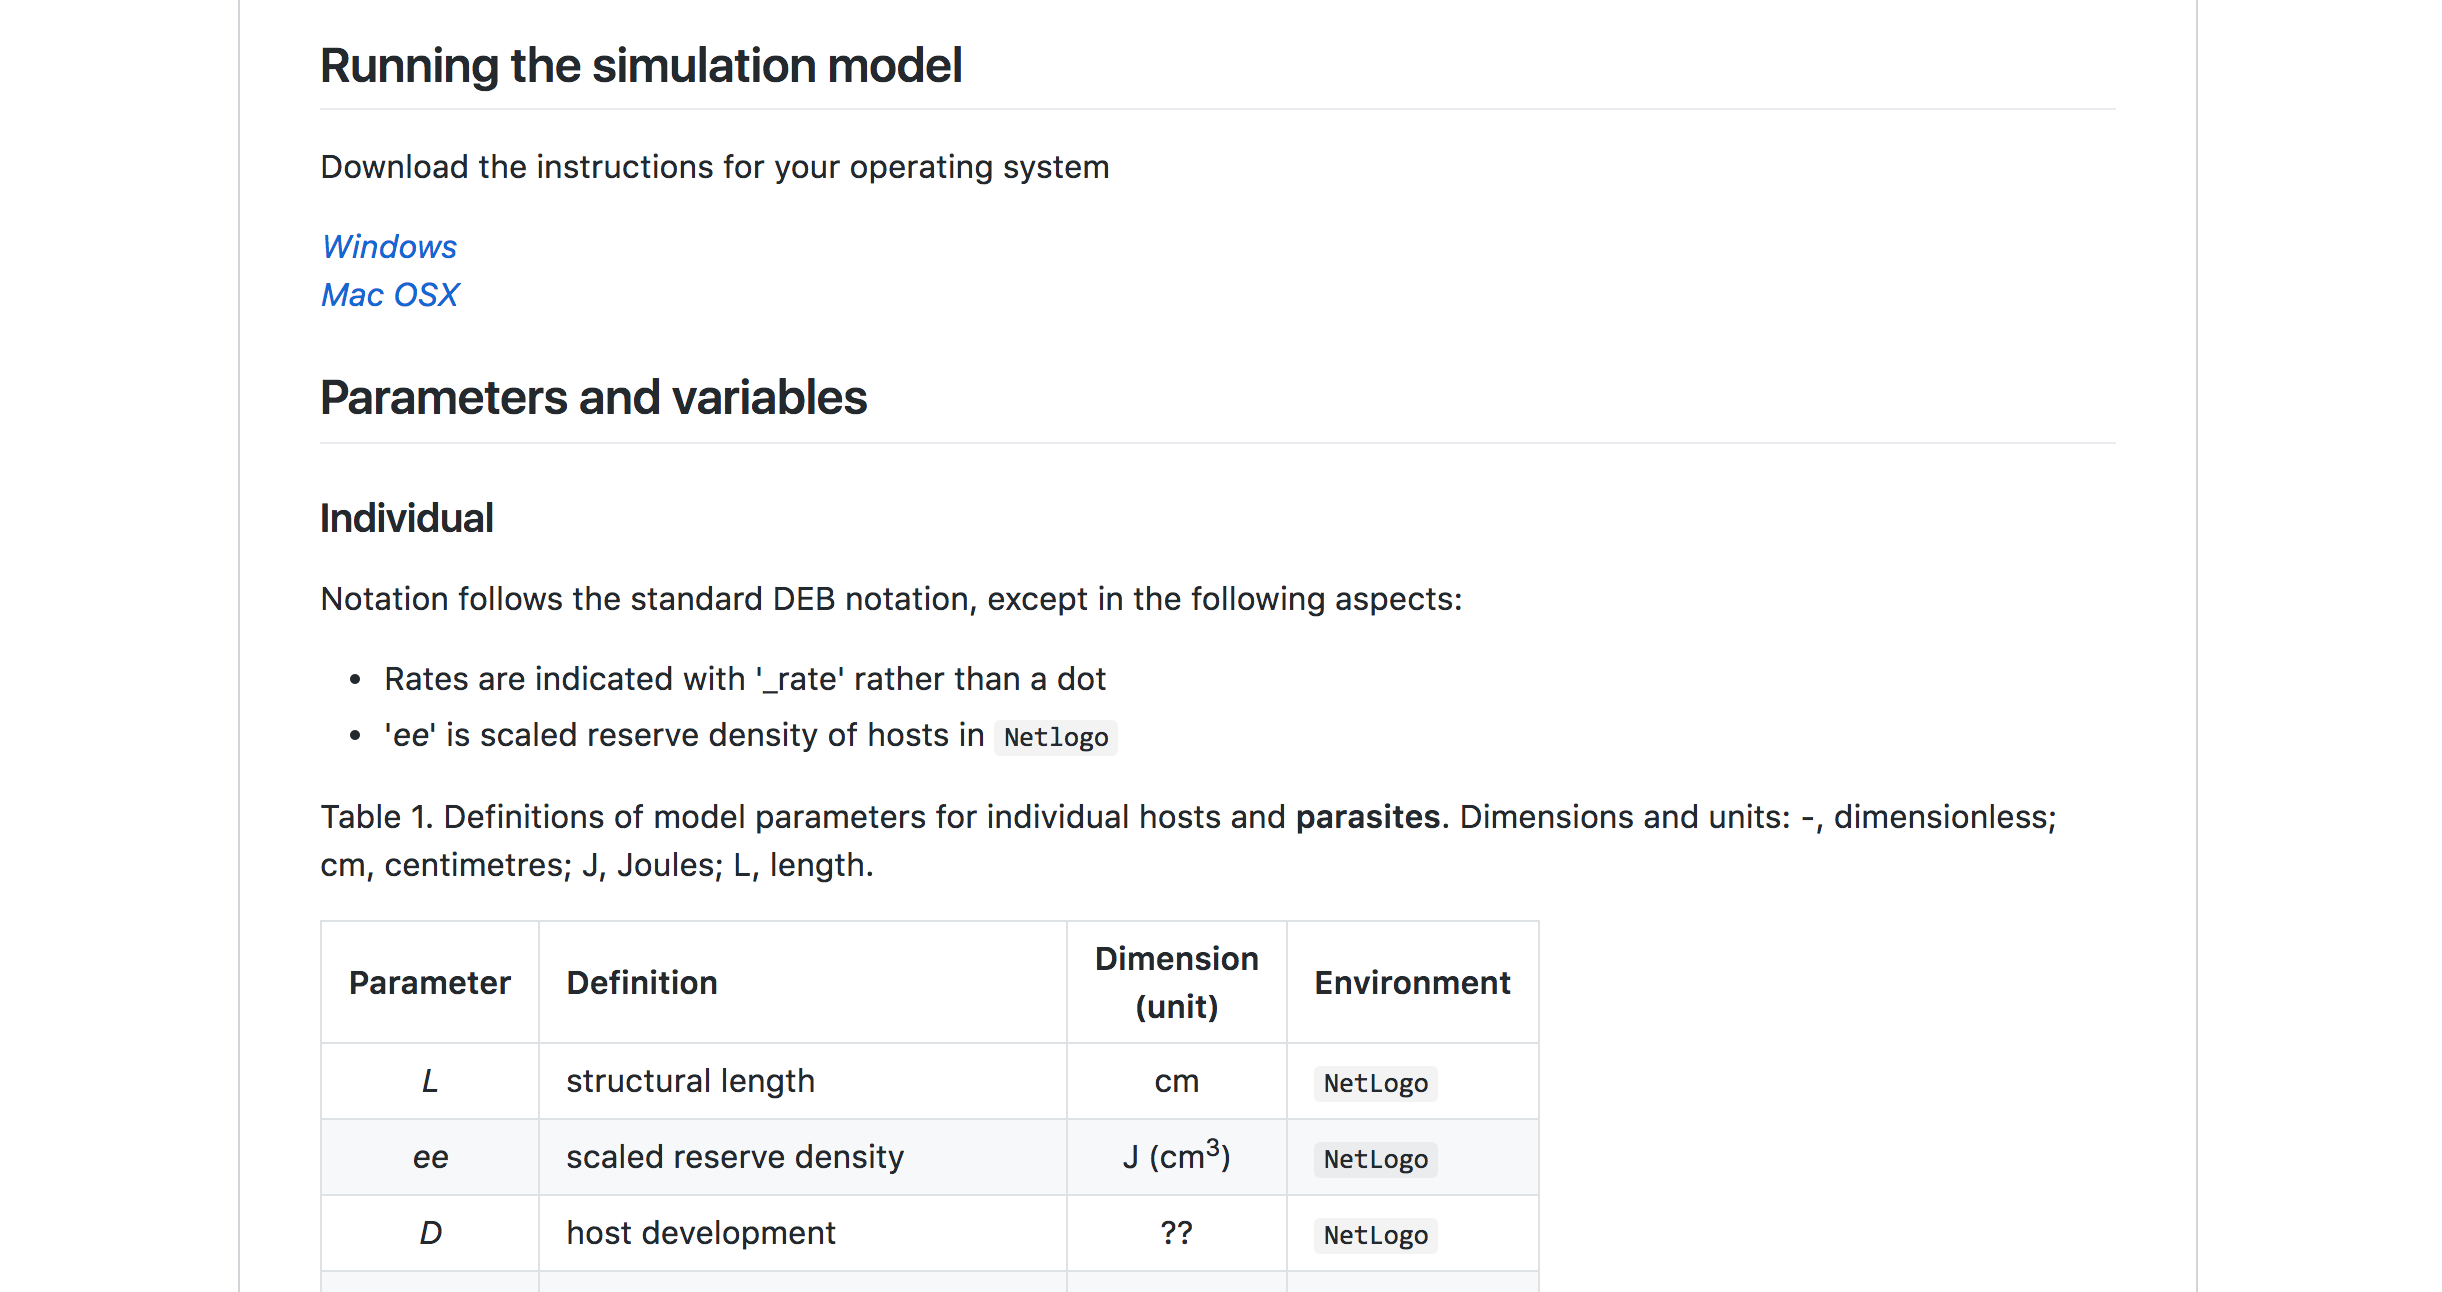
\includegraphics{readme.png}
\caption{Example of a README file}
\end{figure}

\newpage     

\subsection{Using git and Github}\label{using-git-and-github}

We'll be using the command line to talk with git.

\begin{itemize}
\tightlist
\item
  In Mac, this is found in \emph{Applications \textgreater{}
  Terminal}.\\
\item
  In Windows, it's under \emph{Start}, then in the Search line type
  \emph{``cmd''}.
\end{itemize}

~

See these references for a brief intro to using the command line in
\href{https://macpaw.com/how-to/use-terminal-on-mac}{Mac} and
\href{https://www.computerhope.com/issues/chusedos.htm}{Windows}.

~

Here is a brief intro. At least familiarise yourself with these before
the workshop.

\textbf{Useful command line syntax}

\begin{Shaded}
\begin{Highlighting}[]
\BuiltInTok{cd} \CommentTok{# set working dir  }
\BuiltInTok{pwd} \CommentTok{# print current working dir  }
\FunctionTok{ls} \CommentTok{# list files in working dir  }
\FunctionTok{mkdir}\NormalTok{ newfolder }\CommentTok{# make new working dir}
\FunctionTok{touch}\NormalTok{ text.txt }\CommentTok{# create new file }
\end{Highlighting}
\end{Shaded}

\textbf{More useful syntax}

\begin{Shaded}
\begin{Highlighting}[]
\CommentTok{#copy files from _source_ to _destination_. e.g. cp /Users/mydir/README.txt ~/Documents  }
\FunctionTok{cp}\NormalTok{ source destination   }

\CommentTok{# copy all folders, subfolders, and files from _source_ to _destination_  }
\FunctionTok{cp}\NormalTok{ -R source destination  }

\CommentTok{# move files or folders from _source_ to _destination_ (no need for `-R`)  }
\FunctionTok{mv}\NormalTok{ source destination  }

\CommentTok{#move multiple files with the * wildcard, which copies all .rtf files. The tilde (~) symbol is a shortcut for your Home folder, which contains '/Desktop'.}
\FunctionTok{cp}\NormalTok{ ~/Desktop/*.rtf ~/Documents  }

\CommentTok{# rename files }
\FunctionTok{mv}\NormalTok{ ~/Desktop/MyFile.rtf ~/Desktop/MyFile-old.rtf  }
\FunctionTok{cp}\NormalTok{ ~/Desktop/MyFile.rtf ~/Documents/MyFile-old.rtf  }
\end{Highlighting}
\end{Shaded}

\subsection{References}\label{references}

\href{https://git-scm.com/book/en/v2/Getting-Started-Installing-Git}{Installing
git}

\href{https://github.com/}{Sign up to Github}

\href{https://git-scm.com/book/en/v2/Getting-Started-About-Version-Control}{Version
control with git}

\href{https://macpaw.com/how-to/use-terminal-on-mac}{Terminal in Mac}

\href{https://www.computerhope.com/issues/chusedos.htm}{Command line in
Windows}

\subsection{Maintainer}\label{maintainer}

Matt Malishev\\
\href{https://github.com/darwinanddavis}{Github} \textbar{}
\href{https://www.researchgate.net/profile/Matt_Malishev}{Website}\\
matthew.malishev {[}at{]} emory.edu

\printbibliography

\end{document}
